\chapter{Two-body Kinematics}
\label{chapt:kin}
Direct nuclear transfer reactions, as discussed in the previous chapter, can be described in terms of two-body kinematics.  The feature that makes the HELIOS spectrometer unique is the effect that the spectrometer's magnetic field has on the  motion of the reaction products (solenoidal transport) and the way in which the products are measured (detector geometry).  Therefore, in order to have a meaningful discussion of the benefits of HELIOS, it is necessary to introduce the key concepts of reaction kinematics.  This chapter also discusses the specific challenges encountered when measuring reaction in inverse kinematics.  
\section{Basic Principles}
Reaction kinematics form a subset of generalized two-body kinematics.  In the typical %\note{accelerator-target}
setup, a beam of ions of mass $m_1$ are accelerated to a velocity of $v_1$ and bombard stationary target atoms of mass $m_2$.  In ``normal kinematics'' a light ion beam strikes a heavy ion target with $m_1<m_2$.  An example of such a reaction is the $^{28}$Si($d$,$p$) as discussed in Ref~\cite{Mermaz_1971}, in which a deuteron beam strikes a silicon target.  In ``inverse kinematics'' the masses are reversed---a heavy ion beam strikes a light ion target ($m_1>m_2$).  The same ($d$,$p$) reaction on silicon is written in inverse kinematics as $d$($^{28}$Si,$p$).  This is the reaction presented in Ref.~\cite{Lighthall_2010} and discussed in Chapt.~\ref{exp}.
\subsection{Energy}
Before the reaction, given a stationary target and an accelerated ion beam, the total kinetic energy of the two-body system in the laboratory frame is equal to the beam energy $E_1$.  
The total kinetic energy in the center-of-mass system is then given by
\begin{equation}
T_\mathrm{cm}=\frac{m_2}{m_1+m_2}E_1
\label{eq:total-energy}
\end{equation}
where $E_1=\frac{1}{2}m_1v_1^2$ is the kinetic energy of the beam particle.

The system then gains or loses energy depending on the specific reaction energy, referred to as the $Q$-value.  The $Q$-value will be defined here as the change in total energy of the system before and after the reaction in a ground-state transition.  With this definition, the reaction $Q$-value may be calculated as the change in mass.
\begin{equation}
Q=[(m_1+m_2)-(m+M)]c^2
\label{eq:q_value}
\end{equation}
where $Q$ is explicitly the energy \textit{gained} in the reaction\footnote{Some texts define the $Q$-value as the total amount of energy lost in the reaction, in which case $Q^\prime=-Q+E_x$.}.  Here the masses of the reaction products are written as $m$ and $M$, with $m<M$.  In this notation, an endothermic reaction will have a negative $Q$-value.  For transitions to states other than the ground-state, the excitation energy $E_x$ must also be included in calculating %$E_\mathrm{total}$, 
the resultant total kinetic energy in the center-of mass frame.
\begin{equation}
E_\mathrm{total}=T_\mathrm{cm}+Q-E_x
\label{eq:ecmtotal}
\end{equation}

With the energy $E_\textrm{total}$ defined above, the conservation of momentum gives the (non-relativistic) kinetic energy of the ejectile in the center-of-mass system as
\begin{equation}
\begin{split}
E_\mathrm{cm}&=E_\mathrm{total}\frac{M}{m+M}\\
&=\frac{1}{2}m v_0^2
\end{split}
\label{eq:ecm}
\end{equation}
where $v_0$ is the velocity of the ejectile (mass $m$) in the center-of-mass frame.

\subsection{Velocity}
%Two important constants of motion in two-body kinematics are the velocity of the center-of-mass $V_\mathrm{cm}$ and the %velocity of the light ion ejectile %of mass $m$
% in the center-of-mass frame $v_0$. 
The center-of-mass system is defined as the reference frame in which the reactants have equal and opposite momentum vectors.
%In the center-of-mass system, the colliding particles have equal momentum by definition.
In the laboratory system, this center-of-mass has a velocity %of the center-of-mass $V_\mathrm{cm}$  
given by
\begin{equation}
\begin{split}
V_\mathrm{cm}&=v_{1}\frac{m_{1}}{m_{1}+m_{2}}.\\
%&=\sqrt{\frac{2 E_1}{m_1}}\frac{m_{1}}{m_{1}+m_{2}}
\end{split}
\label{Vcm}
\end{equation}
%where $V_1$ and $m_1$ refer to the beam particle and $m_2$ is the target particle.
The velocity of the ejectile (mass $m$) in the center-of-mass frame $v_0$ is given in terms of the total kinetic energy in the center-of-mass $E_\textrm{total}$.  Substituting Eq.~\ref{eq:ecmtotal} into Eq.~\ref{eq:ecm} and solving for $v_0$ yields
\begin{equation}
\begin{split}
v_0%&=\sqrt{\frac{2 E_\mathrm{cm}}{m}}\\
&=\sqrt{\frac{2M(T_\mathrm{cm}+Q-E_x)}{m(m+M)}}.
\end{split}
\label{kin_v0}
\end{equation}

The velocity magnitudes $V_\mathrm{cm}$ and $v_0$ are constants of motion.  Eq.~\ref{Vcm} shows that for a given reaction, $V_\mathrm{cm}$ is fixed by the bombarding energy of the beam particle.  Similarly, Eq.~\ref{kin_v0} shows that $v_0$ is fixed by the reaction $Q$-value and transition energy $E_x$, in addition to the bombarding energy.
These velocities are related to the laboratory velocity by $\vec{v_\mathrm{lab}}=\vec{V_\mathrm{cm}}+ \vec{v_0}$.  The magnitude $v_\mathrm{lab}$ varies as the emission angle $\theta_\mathrm{cm}$ changes.  %This transformation between the laboratory system and the center-of-mass system is visualized graphically in Fig.~\ref{big_kin}.  
With reference to Fig.~\ref{big_kin}, the magnitude $v_\mathrm{lab}$ is readily obtained using the law of cosines
\begin{equation}
v_\mathrm{lab}^2=v_0^2+V_\mathrm{cm}^2-2v_0 V_\mathrm{cm}\cos(180^\circ - \theta_\mathrm{cm}).
\label{eq:law_of_cosines}
\end{equation}
Rewriting in terms energy, one gets
\begin{equation}
\begin{split}
E_\mathrm{lab}%&=\frac{1}{2} m\left[v_0^2+V_\mathrm{cm}^2 +2V_\mathrm{cm}v_0 \cos(\theta_\mathrm{cm})\right]\\
&=E_\mathrm{cm}+\frac{1}{2} m V_\mathrm{cm}^2 +m V_\mathrm{cm}v_0 \cos(\theta_\mathrm{cm}).
\end{split}
\label{elab}
\end{equation}
 %with $v_\mathrm{lab}$ derived from the measured energy, $V_\mathrm{cm}$ set by the beam energy, and $v_0$ is determined by beam energy, the Q-value of the reaction, and the excitation energy.

\begin{figure}%
\centering
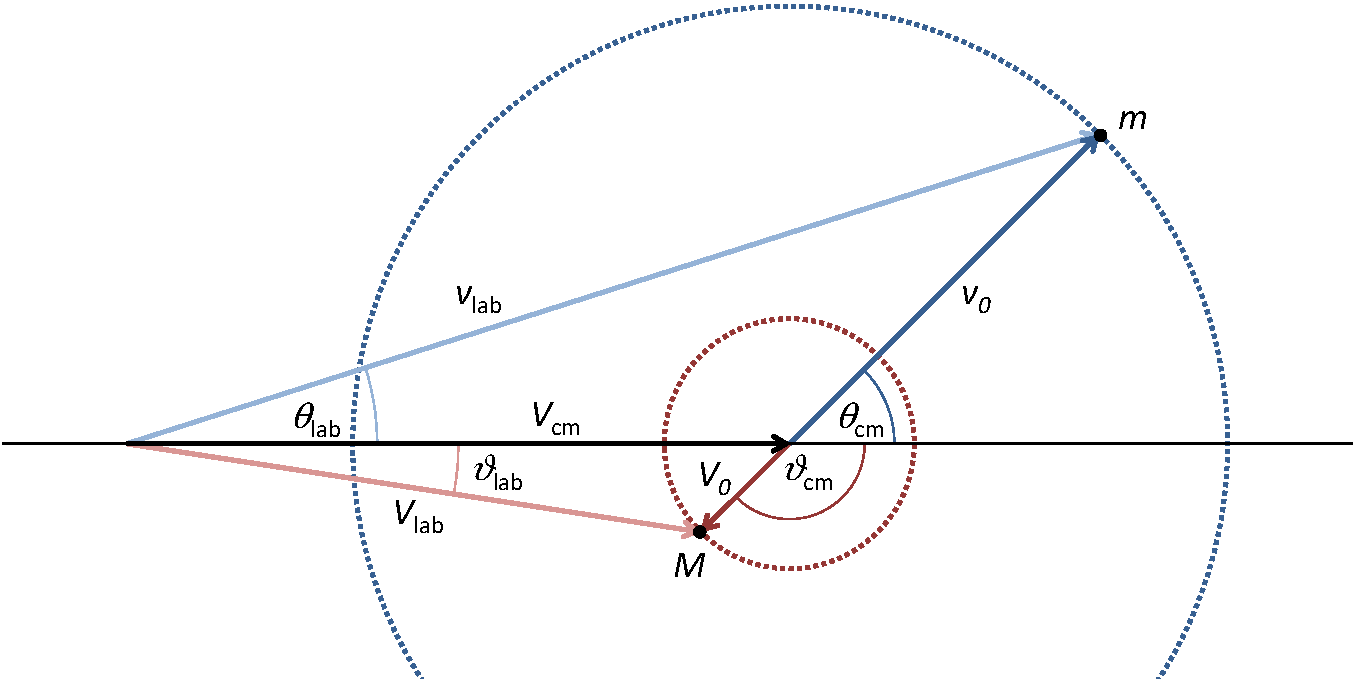
\includegraphics[width=\columnwidth]{kin_fig_3c}
\caption[Transformation of velocities between the laboratory and the center-of-mass systems]{Transformation of velocities between the laboratory and the center-of-mass systems. As the ejection angle of mass $m$ varies (large circle) from $\theta_\mathrm{cm}=0$--$180^\circ$, the particle is scattered at an angle of $\theta_\mathrm{lab}$ such that $\vec{v_\mathrm{lab}}=\vec{V_\mathrm{cm}}+\vec{v_0}$.
  Mass $M$ is ejected such that $\theta_\mathrm{cm}+\vartheta_\mathrm{cm}=180^\circ$.
Adapted from \citet[Fig.~11]{Michalowicz_1967}.}
\label{big_kin}%
\end{figure}

\subsection{Angle}
After the reaction, the ejectile is emitted at an angle in the center of mass $\theta_\mathrm{cm}$ over the range of 0--180$^\circ$.  Due to the conservation of momentum, the ejectile and the heavy recoil are ejected back-to-back in the center-of-mass frame with $\theta_\mathrm{cm}+\vartheta_\mathrm{cm}=180^\circ$% (refer to Fig.~\ref{big_kin})
.  To be consistent with the convention used in most textbooks, the center-of-mass angle $\theta_\mathrm{cm}$ is defined relative to $+V_\textrm{cm}$ direction, as illustrated in Fig.~\ref{big_kin}.  This choice of coordinates is natural in normal kinematics where, in the rest frame of the heavy ion target, the beam is approaching at a velocity of $\approx v_1$.  However, in inverse kinematics %, in the rest frame of the heavy ion beam, 
the target is approaching the heavy ion at a \textit{negative} velocity of $-V_\mathrm{cm}$.  Therefore, in inverse kinematics% To account for this disparity
, the center-of-mass angle is defined as the compliment of the angle shown in Fig.~\ref{big_kin} ($180^\circ-\theta_\mathrm{cm}$).  Thus in both cases, $\theta_\textrm{cm}=0^\circ$ refers to the light ion traveling in the same direction before and after the reaction from the standpoint of the heavy ion.

In the laboratory frame, the extent to which $\theta_\mathrm{lab}$, and in turn $E_\mathrm{lab}$, vary as a function of $\theta_\textrm{cm}$ depends on how $V_\mathrm{cm}$ and $v_0$ compare to one another.  The value of the ratio $K=V_\mathrm{cm}/v_0$ divides the reactions into three classes.  Table~\ref{k_factors5} gives the $K$-values for a number of reactions.

\begin{table*}%[ht]
  \centering
  \begin{tabular}{,....c}		
    \hline
    \multicolumn{1}{c}{\multirow{2}{*}{Reaction}}  &  
    \multicolumn{1}{c}{$Q$-value}  &
    \multicolumn{1}{c}{$E_1/A_1$}  &  
    \multicolumn{1}{c}{$K_\mathrm{g.s.}$}  &  
    \multicolumn{1}{c}{$\theta_\mathrm{max}$} & Ref. \\%\cline{2-6}
    &\multicolumn{1}{c}{(MeV)}  &\multicolumn{1}{c}{(\AMeV)}  &   &\multicolumn{1}{c}{(deg)} & \\
    \hline \hline 
		^{132}\textrm{Sn}(d,p)^{133}\textrm{Sn}  &0.25&  4.78  &  0.01  &  180.0  & \textit{unstable}\\
		^{124}\textrm{Sn}(d,\textrm{He}^3)^{123}\textrm{In}  &-6.61&  14.35  &  0.02  &  180.0  & \cite{Weiffenback_1971}\\
		^{28}\textrm{Si}(d,p)^{29}\textrm{Si}  &6.25&  8.94  &  0.04  &  180.0  & \cite{Mermaz_1971} \\
		^{12}\textrm{B}(d,p)^{13}\textrm{B}  &2.65&  6.24  &  0.10  &  180.0  &\textit{unstable}\\
		d(^{28}\textrm{Si},p)^{29}\textrm{Si}  &6.25&  6.02  &  0.56  &  180.0  & \cite{Lighthall_2010} \\
		d(^{12}\textrm{B},p)^{13}\textrm{B}  &2.65&  6.24  &  0.61  &  180.0  &\cite{Lee_2010,Schiffer_2010}\\
		d(^{132}\textrm{Sn},p)^{133}\textrm{Sn}  &0.25&  4.78  &  0.70  &  180.0  & \cite{Pain_2007,Jones_2007,Pain_2008,Jones_2010} \\
		d(^{124}\textrm{Sn},^3\textrm{He})^{123}\textrm{In}  &-6.61&  13.00  &  1.42  &  44.6  &\textit{proposal}\\
	  \hline
  \end{tabular}
  \caption[Ground-state transition velocity ratios $K_\mathrm{g.s.}$ for a number of reactions]{Ground-state transition velocity ratios $K_\mathrm{g.s.}$ for a number of reactions.  For each reaction, the values are given for both normal and inverse kinematics.  For reactions that have been performed, the beam energy has been selected to match the given reference.}
  \label{k_factors5}
  \end{table*}

\begin{figure}[ht]
\begin{center}
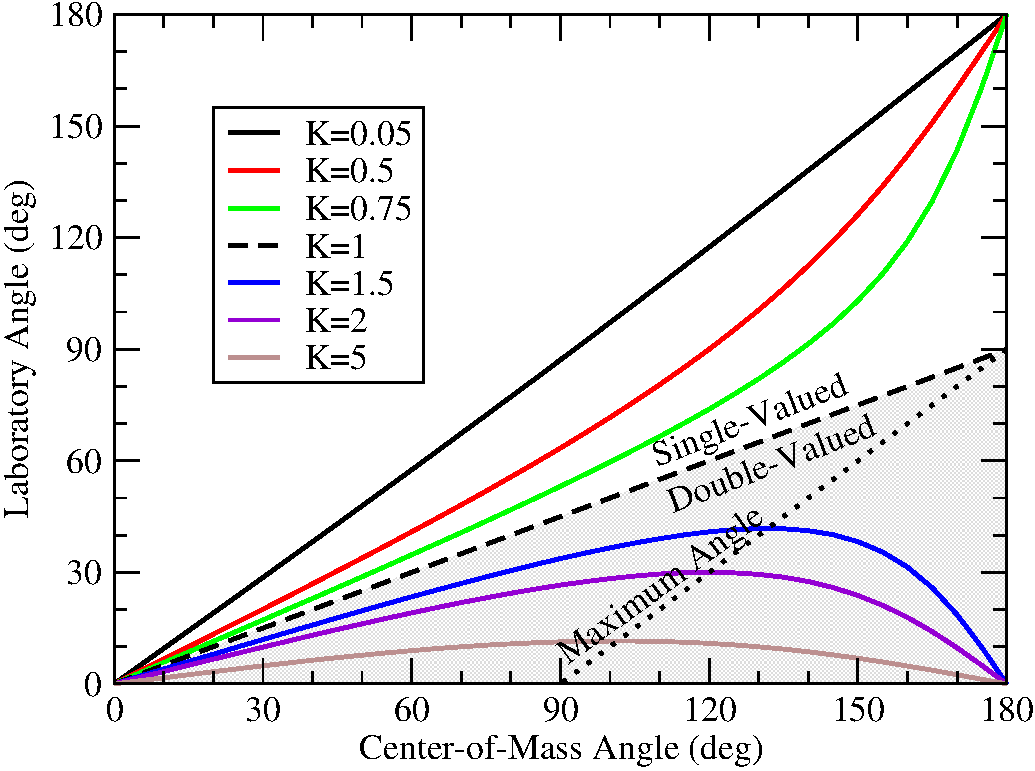
\includegraphics[keepaspectratio,width=\columnwidth,height=0.5\textheight]{angles34}%	
\end{center}
\caption[Transformation of angles between the laboratory and the center-of-mass systems]{Transformation of angles between the laboratory and the center-of-mass systems.  For $K>1$ the transformation is double-valued in the laboratory.  The maximum laboratory angle for such solutions is plotted.  Adapted from \citet[Fig.~9]{Michalowicz_1967}.}%
\label{angles}%
\end{figure}

\subsubsection{$K<1$}
For $K<1$ the laboratory energy $E_\mathrm{lab}$ is a single-valued function of the laboratory angle $\theta_\mathrm{lab}$, with the ejectile being emitted over all laboratory angles.  In the limit of normal kinematics, %the scattered beam ion, which is the light reaction product, is detected.  W
when the beam is much lighter than the target ($m_1 \ll m_2$), the center-of-mass of the reaction system is nearly at rest.  Eq.~\ref{elab} shows that when the velocity ratio $K \ll 1$---that is, when $V_\mathrm{cm} \ll v_0$---the laboratory energy $E_\mathrm{lab}$ begins to lose its dependence on the angle $\theta_\mathrm{cm}$.  This relationship is shown in Fig.~\ref{angles} by the line $K=0.05$ illustrating $\theta_\mathrm{lab}\approx \theta_\mathrm{lab}$.
  
As the ratio $K$ becomes comparable to 1, the reactions enter the realm of inverse kinematics.  The laboratory energy $E_\mathrm{lab}$ varies strongly with angle as the $\cos (\theta_\mathrm{cm})$ term in Eq.~\ref{elab} begins to dominate.  When $V_\mathrm{cm}$ and $v_0$ are more aligned, the energy in the laboratory $E_\mathrm{lab}$ is large compared to the energy in the center-of-mass $E_\mathrm{cm}$.  This corresponds to forward angles in the laboratory; at rearward angles, the inverse is true. 

\subsubsection{$K=1$}
\label{kisone}
$K_\mathrm{g.s.}=1$ is the trivial case, arising in two ways.  First, in elastic scattering, corresponding to $Q=E_x=0$; and second, when $E_x\approx Q+E_1/A_1$.  When no energy is transferred in the reaction, $V_\mathrm{cm}=v_0$ and $\theta_\mathrm{lab}=\frac{1}{2}\theta_\mathrm{cm}$.  The ejectile is emitted in the forward hemisphere only, with $\theta_\textrm{lab} \leq 90^\circ$.  This relationship is shown in Fig.~\ref{angles} by the line $K=1$.
\subsubsection{$K>1$}
For $K>1$, when $v_0<V_\mathrm{cm}$, the ejectile cannot be emitted in the rearward hemisphere.  Thus,  the laboratory energy $E_\mathrm{lab}$ is a double-valued function of the laboratory angle $\theta_\mathrm{lab}$ and the ejectile is emitted over a limited range of angles in the forward hemisphere.  The ejectile has a maximum emission angle in the laboratory given by
\begin{equation}
\theta_\mathrm{max}=\tan^{-1}\left(\frac{1}{\sqrt{K^2-1}}\right)=\sin^{-1}\left(\frac{1}{K}\right)
\label{max_theta}
\end{equation}
The shaded region of Fig.~\ref{angles} illustrates the relationship between $K$ and $\theta_\mathrm{max}$ and Table~\ref{k_factors5} gives $\theta_\mathrm{max}$ for a specific reaction in inverse kinematics.
In such cases, each angle $\theta_\mathrm{lab}$ corresponds to a ``high energy'' solution and a ``low energy'' solution.  The low energy solution corresponds to particles emitted at more forward angles (typically $\theta_\textrm{cm} \lesssim 30^\circ$) in the center-of-mass frame.

In the limiting case of $K \gg 1$, when $V_\textrm{cm} \gg v_0$, Eq.~\ref{elab}  again shows that the laboratory energy $E_\textrm{lab}$ will lose its dependence on the angle $\theta_\textrm{cm}$.  However, in this case, the laboratory velocity is approximately the center-of-mass velocity $v_\textrm{lab}\approx V_\textrm{cm}$.  This is the typical situation for the heavy ion reaction product.  Furthermore, in the limit of inverse kinematics ($m_1\gg m_2$), the velocity of the heavy recoil is then also approximately the incident beam velocity $V_\textrm{lab}\approx V_\textrm{cm} \approx v_1$.  

\section{Inverse Kinematics}
The utility of studying reactions in inverse kinematics is that it provides access to measurements involving heavy isotopes that are unstable against $\beta$-decay.
However, as detailed in the previous section, the transition to inverse kinematics is not simply a reversal of target and beam.  The rapidly changing laboratory quantities that are encountered have serious implications for measurements carried out in inverse kinematics.  In addition, the difficulties associated with a radioactive ion beam must also be considered.  This section discusses several of these challenge.
 
\subsection{Kinematic Compression}
\label{kin_comp}
In inverse kinematics, the center-of-mass of the reaction has a substantial velocity in the laboratory frame.  When the velocity of the light ion reaction product $v_0$ is comparable to the velocity of center-of-mass $V_\mathrm{cm}$, the energies of the emitted light ions are highly angle-dependent.  When these velocities are anti-aligned (forward center-of-mass angles), the laboratory energy is significantly smaller than in normal kinematics.  This also has the effect of compressing the relative spacing between energy levels at a given $\theta_\mathrm{lab}$.

\subsubsection{Compression Coefficient}
The separation between two energy levels in the laboratory frame is defined here as $\Delta E_\mathrm{lab}=(E_\mathrm{lab}-E_\mathrm{lab}^\prime)$.  Starting with Eq.~\ref{elab} and holding $V_\mathrm{cm}$ and $\theta_\mathrm{cm}$ constant, the energy separation in the laboratory at a fixed emission angle is given by
\begin{equation}
\begin{split}
\Delta E_\mathrm{lab}
&=\Delta E_\mathrm{cm}+mV_\mathrm{cm}\Delta v_0 \cos(\theta_\mathrm{cm})
\end{split}
\label{eq:delta_e2}
\end{equation}
The energy separation in the center-of-mass frame is given by
\begin{equation}
\begin{split}
\Delta E_\mathrm{cm}
&=\frac{1}{2}m \Delta (v_0)^2\\
&=\frac{1}{2}m (v_0+v_0^\prime)\Delta v_0
\end{split}
\label{eq:delta_ecm}
\end{equation}
The ratio of the separation of the energy levels in the laboratory $\Delta E_\mathrm{lab}$ to that in center-of-mass will be defined here as the ``compression coefficient''
\begin{equation}
\begin{split}
\frac{\Delta E_\mathrm{lab}}{\Delta E_\mathrm{cm}}
&=\frac{\Delta E_\mathrm{cm}+mV_\mathrm{cm}\Delta v_0 \cos(\theta_\mathrm{cm})}{\frac{1}{2}m (v_0+v_0^\prime)\Delta v_0}\\
&=1+\frac{2V_\mathrm{cm}\cos(\theta_\mathrm{cm})}{(v_0+v_0^\prime)}\\
&=1+\frac{2 K \cos(\theta_\mathrm{cm})}{(1+v_0^\prime/v_0)}
\end{split}
\label{eq:compress}
\end{equation}
and is identically equal to $1$ at $\theta_\mathrm{cm}=90^\circ$.  For reactions in normal kinematics, with $K \ll 1$, this effect is suppressed and $\Delta E_\mathrm{lab}/\Delta E_\mathrm{cm}\approx 1$ for all angles.  In both normal and inverse kinematics, at rearward emission angles ($\theta_\mathrm{cm}>90^\circ$) the effect causes an increase of the energy spacing ($\Delta E_\mathrm{lab}/\Delta E_\mathrm{cm}> 1$).  
However, in order to differentiate the angular distributions associated with different angular momentum transfers, it is necessary to measure the reactions at forward angles ($\theta_\textrm{cm} \lesssim 30^\circ$).  This region of interest is where the effect of kinematic compression is the most dramatic.  
In cases when the $K$-value of the reaction is $>1$, meaning the laboratory energy $E_\mathrm{lab}$ is a double-valued function of the laboratory angle $\theta_\mathrm{lab}$, the value of $\Delta E_\mathrm{lab}/\Delta E_\mathrm{cm}$ is negative for the low energy solution.  In some cases,  the low energy solution will also see an enhancement in the energy level spacing ($\Delta E_\mathrm{lab}/\Delta E_\mathrm{cm}< -1$) at the most forward laboratory angles.

\subsubsection{Example}
Fig.~\ref{sn-plots} shows calculated plots of energy $E_\textrm{lab}$ vs. angle $\theta_\textrm{lab}$ %in the laboratory 
for the ($d$,$p$) reaction on $^{132}$Sn at 4.78\,\AMeV.  This bombarding energy is chosen to match the measurement of \citet{Jones_2010}.  This reaction is a benchmark measurement for inverse kinematics, not only because of the importance of the physics associated with the measurement (see Chapt.~\ref{astro}), but also because of the difficulty of the measurement.  In the figure, fictitious energy levels have been selected such that $\Delta E_x=1.0$\,MeV to illustrate kinematic compression.

$^{132}$Sn is unstable against $\beta$-decay with a half-life of $T_{1/2}=39.7$\,s.  Therefore it is impossible to make a $^{132}$Sn target for a reaction study in normal kinematics.  However, if it \textit{were} possible to perform this reaction in normal kinematics (left panel), the ground state transition would have a velocity ratio of $K_\mathrm{g.s.}=0.01$ and at $\theta_\mathrm{cm}=10^\circ$ the ``compression'' coefficient is $1.01$.  In inverse kinematics, the ground state transition has a velocity ratio of $K_\mathrm{g.s.}=0.70$ and at $\theta_\mathrm{cm}=10^\circ$ the compression coefficient is $0.30$.  Furthermore, in inverse kinematics, for excitation energies $E_x \gtrsim (Q+E_1/A_1)$, in this case $\approx 5$\,MeV, the energy solution is double-valued ($K>1$).  

\begin{figure}[ht]
\centering
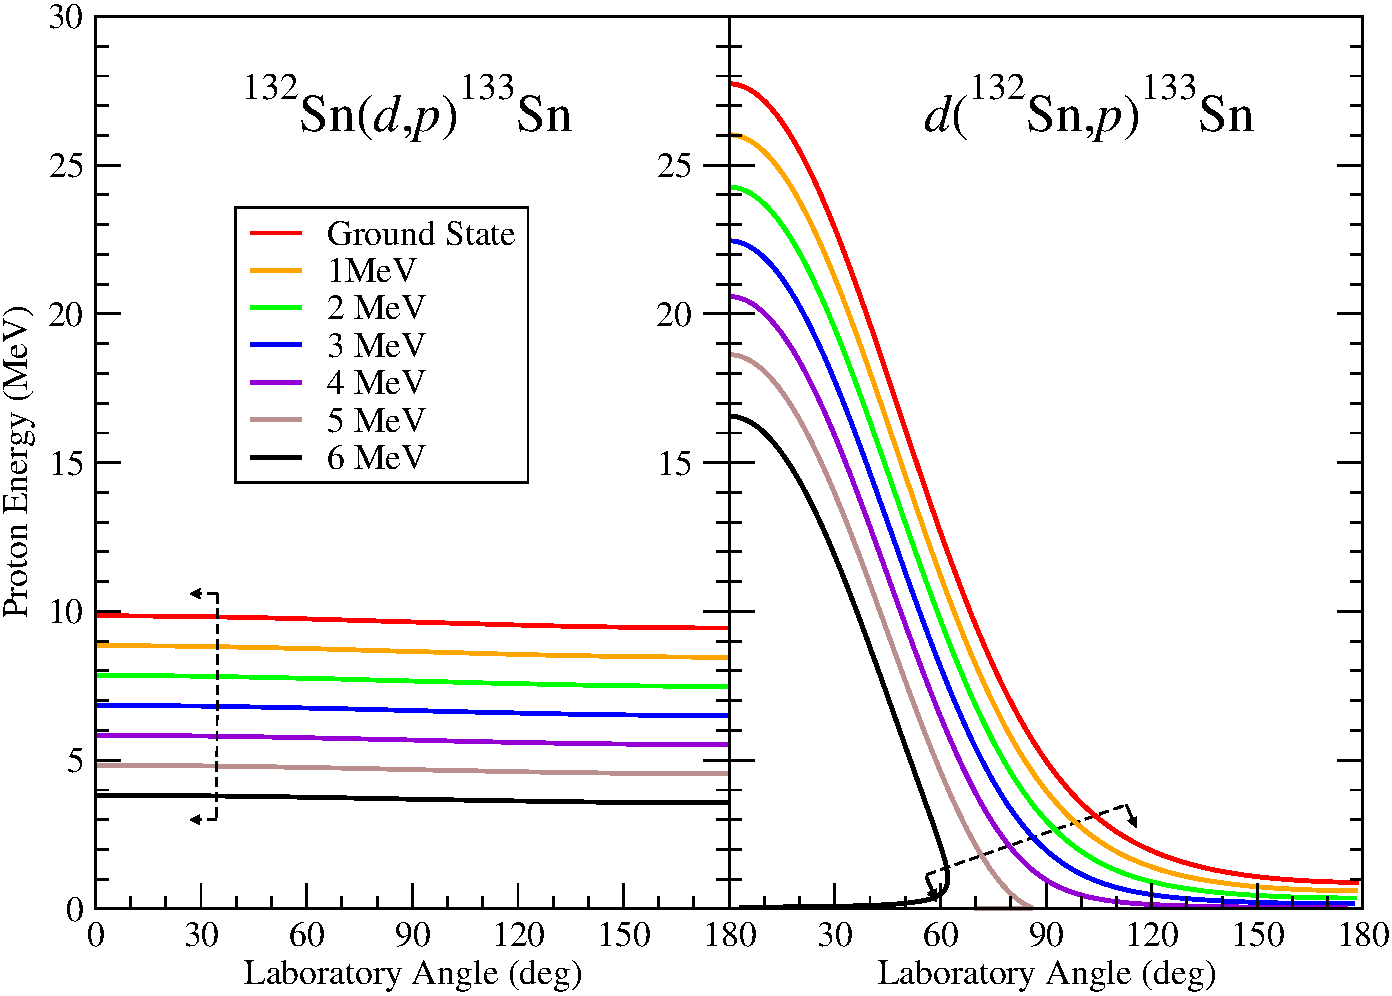
\includegraphics[width=\columnwidth,height=0.45\textheight,keepaspectratio]{sn132-plots3b}
\caption[Illustration of kinematic compression]{Illustration of kinematic compression.  In normal kinematics (left, $K_\mathrm{g.s.}=0.01$), the energy level spacing approximately constant and equal to the spacing in the center-of-mass.  In inverse kinematics (right, $K_\mathrm{g.s.}=0.70$), the energy spacing is dramatically compressed at forward angles, corresponding to emission in the rearward hemisphere.  The dashed lines indicate the approximate position of $\theta_\mathrm{cm}=35^\circ$, with the arrows indicating forward angles in the center-of-mass.  Note the laboratory energy $E_\mathrm{lab}$ becomes double-valued in inverse kinematics for $E_x > 5$\,MeV.}%
\label{sn-plots}%
\end{figure}

\subsection{Kinematic Broadening}
\label{kin_broad}
The effect of kinematic compression emphasizes the need for high-resolution energy measurements in inverse kinematics.  In addition, due to the strong dependence of the light recoil energy $E_\mathrm{lab}$ on laboratory angle $\theta_\mathrm{lab}$, it becomes essentially important to have precise angle measurement.  % in inverse kinematics.
Even in a system with perfect energy resolution ($\delta E_\mathrm{lab}=0$), the range of angles covered by a finite detector element $\delta \theta_\mathrm{lab}$ corresponds to a range in measured energy; thus leading to a reduced measured energy resolution.  This relationship is illustrated in Fig.~\ref{error_fig}.  For example, in the $d$($^{132}$Sn,$p$) reaction discussed above, at $\theta_\mathrm{cm}=10^\circ$ ($\theta_\mathrm{lab}=149^\circ$) the rate-of-change (\textit{i.e.} slope) of the ground state transition in the laboratory is $dE_\mathrm{lab}/d\theta_\mathrm{lab}=41$\,keV/deg; at $\theta_\mathrm{lab}=90^\circ$ this value increases to 168\,keV/deg.  This unavoidable feature is referred to as the ``kinematic broadening'' of the %center-of-mass
 energy resolution~\cite{Winfield_1997}.  Put another way, due to the covariance between energy and angle, the energy resolution %in the center-of-mass frame 
 can be limited by angular resolution and vice-versa.  This effect is discussed below and demonstrated in Fig.~\ref{kin_broad_fig}.
 
\begin{figure}%
%\includegraphics[width=\columnwidth]{error_fig}\\%
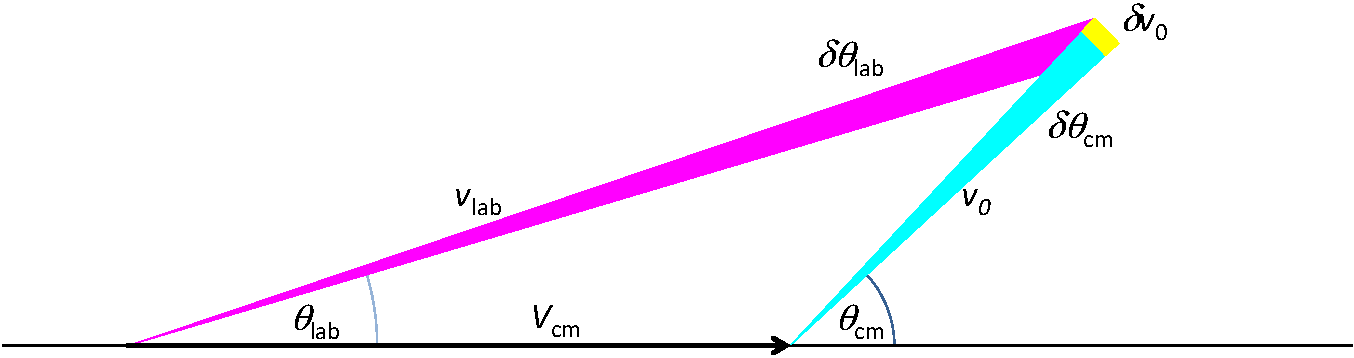
\includegraphics[width=\columnwidth]{error_fig2}%
\caption[Illustration of kinematic broadening]{Illustration of kinematic broadening.  For a fixed measurement of energy, an uncertainty in angle $\delta \theta_\mathrm{lab}$ leads to an uncertainty in both the (derived)  angle $\delta \theta_\mathrm{cm}$ and the energy (via $\delta v_0$).}%
\label{error_fig}%
\end{figure} 

\subsubsection{Resolution Propagation}
\label{res_prop}
The uncertainty of the measured quantity $\theta_\mathrm{lab}$ may lead to a kinematic broadening of the measured quantity $E_\mathrm{lab}$, as mentioned, but it also effects the derived quantities % in center-of-mass frame 
$E_\mathrm{cm}$ and $\theta_\mathrm{cm}$.  To see exactly how the measurement uncertainties effect the derived results, it is necessary to  perform an error analysis. 
%Through the region of interest, the center-of-mass angle changes more rapidly than the laboratory angle.  Therefore uncertainty in the center-of-mass angle is larger than the uncertainty in the laboratory angle.  The broadening of uncertainty lowers the final resolution of the center-of-mass energy spectrum.  This feature will always be present in an experiment measuring angle and energy to reconstruct inverse kinematics.
Solving Eq.~\ref{elab} for $E_\mathrm{cm}$ and rewriting in terms of the measured quantities $E_\mathrm{lab}$ and $\theta_\mathrm{lab}$ (this substitution is derived in Eq.~\ref{elab_of_vpara}) yields

\begin{equation}
\begin{split}
E_\mathrm{cm}&=E_\mathrm{lab}-\frac{1}{2} m V_\mathrm{cm}^2 -m V_\mathrm{cm}v_0 \cos(\theta_\mathrm{cm})\\
&=E_\mathrm{lab}+\frac{1}{2} m V_\mathrm{cm}^2 -m V_\mathrm{cm}v_\mathrm{lab} \cos(\theta_\mathrm{lab})\\
&=E_\mathrm{lab}+\frac{1}{2} m V_\mathrm{cm}^2 - V_\mathrm{cm}(\sqrt{2mE_\mathrm{lab}})\cos(\theta_\mathrm{lab})\\
\end{split}
\label{ecm3}
\end{equation}
Given this relationship, the uncertainty in $E_\mathrm{cm}$ due to the uncertainty in $E_\mathrm{lab}$ and $\theta_\mathrm{lab}$ can be calculated using the generalized error propagation equation~\cite{Bevington_2003,Drosq_2007}.
\begin{equation}
\begin{split}
\left(\delta E_\mathrm{cm}\right)^2&=\left(\frac{\partial E_\mathrm{cm}}{\partial E_\mathrm{lab}}\right)^2\left(\delta E_\mathrm{lab}\right)^2+\left(\frac{\partial E_\mathrm{cm}}{\partial \theta_\mathrm{lab}}\right)^2\left(\delta \theta_\mathrm{lab}\right)^2
%\\&\qquad
+2\left(\frac{\partial E_\mathrm{cm}}{\partial E_\mathrm{lab}}\right) \delta E_\mathrm{lab} \left(\frac{\partial E_\mathrm{cm}}{\partial \theta_\mathrm{lab}}\right)\delta \theta_\mathrm{lab}\\
\end{split}
\label{eq:delta_z4}
\end{equation}
The first two terms in this expression are the individual contributions of the two measured quantities, which are always positive.  The third term is the contribution of the covariance between the two quantities and can (mathematically) take on positive and negative values.  Each term is weighted by a partial derivative.  The weight for the uncertainty in energy $\delta E_\mathrm{lab}$ is given by
\begin{equation}
\begin{split}
\frac{\partial E_\mathrm{cm}}{\partial E_\mathrm{lab}}&=1-mV_\mathrm{cm}\cos(\theta_\mathrm{lab}) \sqrt{\frac{m}{2E_\mathrm{lab}}}
\end{split}
\label{eq:delta_E}
\end{equation}
and the weight for the uncertainty in angle $\delta \theta_\mathrm{lab}$ is given by
\begin{equation}
\begin{split}
\frac{\partial E_\mathrm{cm}}{\partial \theta_\mathrm{lab}}&=V_\mathrm{cm}\sqrt{2mE_\mathrm{lab}}\sin(\theta_\mathrm{lab}).
\end{split}
\label{eq:delta_theta}
\end{equation}

Thus using this technique, the contribution of the individual uncertainties in the measured quantities can be calculated.  Unless otherwise specified, the value of the uncertainties are characterized in terms of the full-width at half maximum (FWHM) $\Gamma$, as opposed to the standard deviation $\sigma$; the two are related by $\Gamma=2.35\sigma$.   Table~\ref{error_prop} shows the results of these calculations for a number of reactions in a manner similar to that presented by \citet{Winfield_1997}.  Following Ref.~\cite{Winfield_1997}, the contributions are calculated assuming measurement uncertainties of $\delta E_\mathrm{lab}=40$\,keV~FWHM, $\delta \theta_\mathrm{lab}=0.54^\circ$~FWHM and an uncertainty in the beam energy (discussed below) of 0.14\%.  However in Ref.~\cite{Winfield_1997}, the individual contributions are added in quadrature, neglecting the effects of the covariance of the measured quantities.  The two rightmost columns in Table~\ref{error_prop} show the sum of the uncertainties added quadratically $\Sigma_\textrm{quad}$ and the sum including the covariation term $\Sigma_\textrm{covar}$.  As expected, this contribution has little effect in normal kinematics where the covariance between $E_\mathrm{lab}$ and $\theta_\mathrm{lab}$ is negligible.  However, in inverse kinematics the contribution of the covariance is significant.  The last two rows of Table~\ref{error_prop} show that in some cases (when $K>1$), the contribution of covariance tends to improve the $Q$-value resolution.

\begin{table*}[hb]
  \centering
  \begin{tabular}{,.....rr}		
    \hline
    \multicolumn{1}{c}{\multirow{2}{*}{Reaction}}  &
    \multicolumn{1}{c}{$E_1/A_1$}  &
    \multicolumn{1}{c}{$\theta_\textrm{lab}$} & 
    \multicolumn{3}{c}{Origin of contribution}  &
    \multicolumn{2}{c}{$\delta E_\textrm{cm}$}  \\  \cline{4-6}
    &\multicolumn{1}{c}{(\AMeV)}&
    \multicolumn{1}{c}{(deg)} & 
    \multicolumn{1}{c}{$\delta \theta_\mathrm{lab}$}  &  
    \multicolumn{1}{c}{$\delta E_\textrm{lab}$} & 
    \multicolumn{1}{c}{$\delta E_1$} & 
    \multicolumn{1}{c}{$\Sigma_\mathrm{quad}$} &
    \multicolumn{1}{c}{$\Sigma_\mathrm{covar}$} \\
    \hline \hline 
		^{132}\textrm{Sn}(d,p)^{133}\textrm{Sn} 	 &4.78 & 9.9 &0 & 40 & 0 & 40 & 40\\
		^{124}\textrm{Sn}(d,\textrm{He}^3)^{123}\textrm{In} 	 &14.35 & 9.8 &2 & 39 & 0 & 39 & 41\\
		^{28}\textrm{Si}(d,p)^{29}\textrm{Si} 	 & 8.94 & 9.6 &3 & 38 & 0 & 39 & 41\\
		^{12}\textrm{B}(d,p)^{13}\textrm{B}   &6.24 & 9.1 &4 & 36 & 0 & 37 & 40\\
		d(^{28}\textrm{Si},p)^{29}\textrm{Si} 	 &6.02 & 157.9 &31 & 85 & 8 & 91 & 116\\
		d(^{12}\textrm{B},p)^{13}\textrm{B} 	 &6.24 & 155.2 &25 & 93 & 7 & 97 & 118\\
		d(^{132}\textrm{Sn},p)^{133}\textrm{Sn}	 &4.78 & 149.0 &22 & 111 & 7 & 113 & 133\\
		d(^{124}\textrm{Sn},^3\textrm{He})^{123}\textrm{In} 	 &13.00 & 21.5 &87 & 72 & 55 & 126 & 57\\
		p(^{77}\textrm{Kr},d)^{76}\textrm{Kr}  	 &30.00 & 15.1 &118 & 54 & 85 & 156 & 106\\
		\hline
  \end{tabular}
  \caption[Calculated contributions to the uncertainty of $E_\textrm{cm}$ for a number of reactions]          {Calculated contributions to the uncertainty of $E_\textrm{cm}$ for a number of reactions.  Values are calculated in keV~FWHM for $\theta_\mathrm{cm} = 10^\circ$, with $\delta E_\mathrm{lab}=40$\,keV, $\delta \theta_\mathrm{lab}=0.54^\circ$ and $\delta E/E=0.14$\%.  The quadratic sum $\Sigma_\mathrm{quad}$ and the sum including the covariant term $\Sigma_\mathrm{covar}$ are given. Adapted from Ref.~\cite[Table~2]{Winfield_1997}.}
  \label{error_prop}
  \end{table*}

\subsection{Discussion}
In normal kinematics, the dominant contribution to the uncertainty of the center-of-mass energy $\delta E_\mathrm{cm}$ (\textit{i.e.} the $Q$-value resolution) is the intrinsic energy resolution of the detectors.  In addition, the energy separation between excited states in the laboratory is nearly the same as that in the center-of-mass frame.  However, in inverse kinematics, the significant covariance between $\theta_\mathrm{lab}$ and $E_\mathrm{lab}$ due to the kinematics of the reaction tends to broaden the resolution of the measured (and derived) quantities.  The net result of measuring reactions in inverse kinematics at forward center-of-mass angles is that separate energy levels are compressed together and are measured with broadened resolution, which tends to blur the states together.  These effects are illustrated in Fig.~\ref{kin_broad_fig}.  To address these problems, one approach is to implement a large detector array with excellent angle resolution.  This method has the disadvantage that it requires a complicated assortment of detectors and electronics.  However, the challenges encountered in conducting reactions in inverse kinematics do not completely preclude their study.  Chapt.~\ref{standards} describes two ``traditional'' approaches to measuring transfer reactions with exotic beams.     Another approach is to measure the nuclear reactions in a new way that avoids or suppresses kinematic compression and kinematic broadening.  The Helical Orbit Spectrometer (HELIOS) at Argonne National Laboratory, discussed in Chap.~\ref{HELIOS_Concept} and on, provides such an approach.

\begin{figure}%
\centering
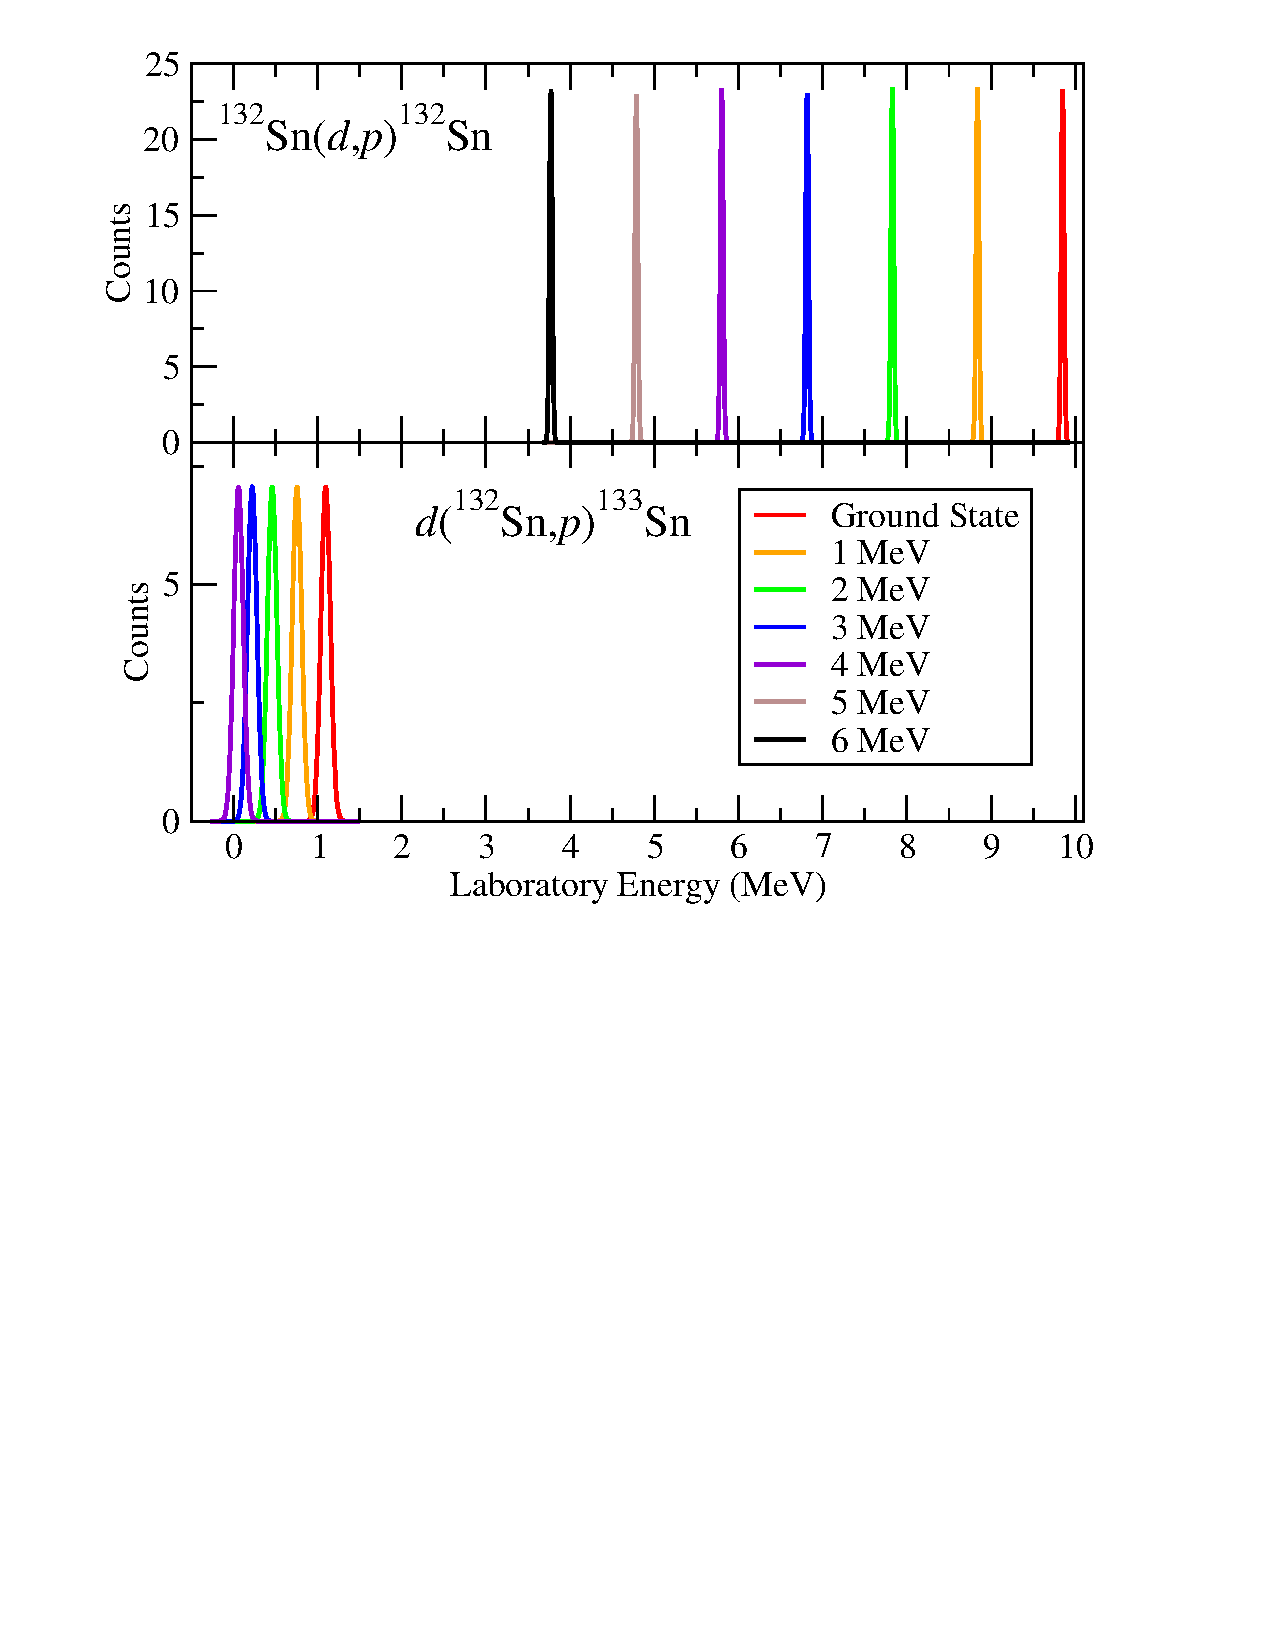
\includegraphics[width=\columnwidth,height=0.45\textheight,keepaspectratio]{sn132-plots4}
\caption[Illustration of the combined effect of kinematic compression and kinematic broadening]{Illustration of the combined effect of kinematic compression and kinematic broadening.  Calculated energy spectra are plotted for a fixed laboratory angle corresponding to at $\theta_\mathrm{cm}=10^\circ$, consistent with Fig.~\ref{sn-plots} and Table~\ref{error_prop}.  In normal kinematics (top, $\theta_\mathrm{lab}=9.9^\circ$), the energy level spacing approximately constant and equal to the spacing in the center-of-mass.  These states are plotted assuming an energy resolution of 40\,keV~FWHM.  In inverse kinematics (bottom, $\theta_\mathrm{lab}=149^\circ$), the energy spacing is dramatically compressed and the resolution is broadened to 133\,keV~FWHM.  States above $E_x > 5$\,MeV are not emitted in the rearward hemisphere.}%
\label{kin_broad_fig}%
\end{figure}

\subsection{Other Contributions}
\label{other_contrib}
\subsubsection{Intrinsic Width}
The discussion of resolution propagation presented above assumes that the states being measured have a natural width much smaller than the measurement uncertainty.  The intrinsic shape of an excited state is a Lorenzian distribution with a width given by the Heisenburg uncertainty principle
\begin{equation}
\Delta E \Delta t \leq \hbar
\label{eq:heisenburg}
\end{equation}
(here the standard symbol for uncertainty $\Delta$ has been used)\cite{Satchler_1990}.  If $\tau$ is the lifetime of the excited state, the width $\Gamma$ is given by 
\begin{equation}
\Gamma \simeq \hbar/\tau.
\label{eq:width}
\end{equation}
For example, the first-excited state in $^{29}$Si has a lifetime of $\tau=290$\,fs, which corresponds to a characteristic width of 2.3\,meV (\textit{milli}-electronvolts); this is a typical value for a bound nuclear excited state.  Therefore, under realistic conditions, the shape and width of measured excited states is dominated by the intrinsic detector resolution and, depending on the reaction, kinematic effects.  
In addition to the intrinsic resolution properties of the detector system, an important contribution to the $Q$-value resolution is the quality of the incident beam and the thickness of the target.

\subsubsection{Beam Energy}
The beam energy $E_1$ enters into the calculation of $E_\mathrm{cm}$ via the center-of-mass velocity $V_\mathrm{cm}$.  Rewriting $V_\mathrm{cm}$ in terms of $E_1$ yields
\begin{equation}
\begin{split}
V_\mathrm{cm}&=\sqrt{\frac{2E_1}{m_1}}\left(\frac{m_1}{m_1+m_2}\right).
\end{split}
\label{vcm2}
\end{equation}
Substituting this expression into Eq.~\ref{ecm3} and differentiating gives the contribution weight of the beam energy uncertainty $\delta E_1$ to the $Q$-value resolution.
\begin{equation}
\begin{split}
\frac{\partial E_\mathrm{cm}}{\partial E_1}&=\frac{m}{m_1}\left(\frac{m_1}{m_1+m_2}\right)^2-m(v_\mathrm{lab} \cos(\theta_\mathrm{lab}))\left(\frac{m_1}{m_1+m_2}\right)\sqrt{\frac{1}{2m_1E_1}}
\end{split}
\label{eq:delta_vcm}
\end{equation}
The value of $\delta E_1$ depends on many factors, such as method of beam production.  However, for an example with a stable beam, Fig.~\ref{beam_energy} shows  several measurements of the beam energy $E_1$ and the uncertainty in the beam energy $\delta E_1$ over the first five days of the  $d(^{28}\textrm{Si},p)^{29}\textrm{Si}$ experiment in Ref.~\cite{Lighthall_2010}.
The beam energy had a nominal value of 168\,MeV (6\,\AMeV) with a measured value of $E_1=168.53 \pm 0.24$\,MeV. %using the $\chi^2$ minimization method with $\delta E_1=\sigma_{E_1}=240$\,keV.
  This level of uncertainty corresponds to a relative uncertainty in the beam energy of $\delta E_1/E_1=0.14$\%.  The contribution of this uncertainty is shown in the sixth column of Table~\ref{error_prop}.  For unstable beams, the uncertainty in the beam energy will typically be higher than that for stable beams, although to what degree this is so depends on the method of beam production.

\begin{figure}[t]
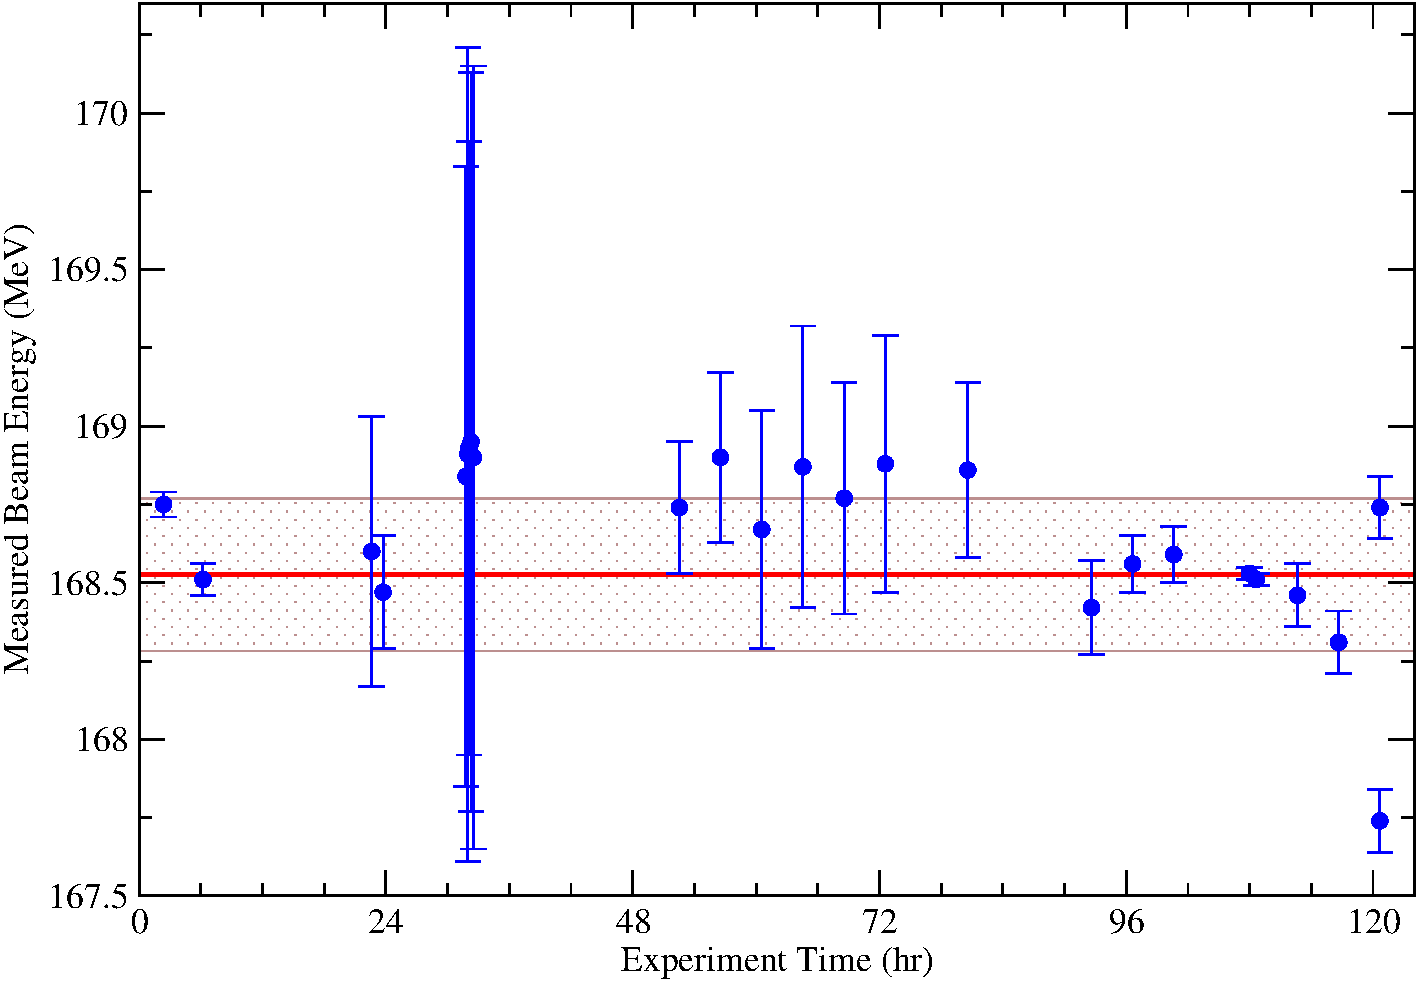
\includegraphics[width=\columnwidth]{beam_energy2}%
\caption[Beam energy and errors as measured during the $d$($^{28}$Si,$p$) experiment]{Beam energy and errors as measured during the $d$($^{28}$Si,$p$) experiment.  Both quantities measured by the ATLAS time-of-flight during the experiment reported in Ref.~\cite{Lighthall_2010}.  The horizontal line is the calculated average beam energy with $\pm 1 \sigma$ window.}%
\label{beam_energy}%
\end{figure}

\subsubsection{Beam Size}
Depending on the beam production technique, the heavy ion beam may have a substantial lateral extent---on the order of 1--5\,mm---at the target plane.  This transverse area is referred to as the beam spot size.  An increase in the uncertainty of the transverse extent of the interaction area between the beam and the target $\delta x$, $\delta y$ leads to a smearing of the measured scattering angle.  Fig.~\ref{beam_spot}(a) shows the effect of a finite beam spot size.  A similar effect, the effect of a misalignment of the beam, will also produce an error in determining the angle.  The contribution of this effect is discussed in Chapt.~\ref{simulation}.

\begin{figure}[t]%
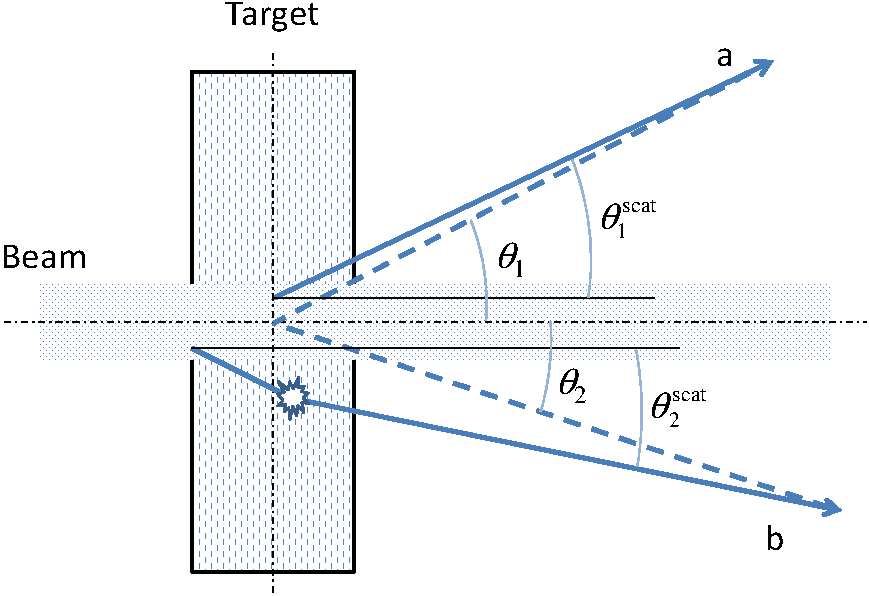
\includegraphics[keepaspectratio,width=\columnwidth,height=0.45\textheight]{beam_target}%
\caption[Illustration of the effect of beam spot size and target thickness on the light ejectile]{Illustration of the effect of beam spot size and target thickness on the light ejectile.  (a) The nuclear reaction occurs off the nominal beam axis, resulting in a disparity between the actual scattering angle $\theta_1^\textrm{scat}$ and the detected scattering angle $\theta_1$.  (b) The nuclear reaction occurs near the front of the target and the light ejectile scatters again while passing through the target.  Adapted from Ref.~\cite[Fig.~7]{Winfield_1997}}%
\label{beam_spot}%
\end{figure}

\subsubsection{Target Effects}
The light ions classically available for accelerated beams are not necessarily readily available, or perhaps practical, for use as target.  While most electrostatic accelerator facilities can produce pure beams of light ions, a solid cryogenic hydrogen target for high-resolution measurements, for instance, is impossible.  Instead, hydrogen beams are replaced with targets made of polyethylene (C$_2$H$_4$)$_{n}$ or polypropylene (C$_3$H$_6$)$_{n}$.  Similarly, the inverse kinematics analog of a deuteron beam could be a deuterated polyethylene (C$_2$D$_4$)$_{n}$ target.

The relatively low intensity beams achievable with most radioactive isotopes can be compensated for, in part, by the use of thicker targets.  However in a thicker target, the nuclear reactions can occur at a variety of depths.  When the bombarding beam consists of heavy ions, the energy loss associated with passing through the target $dE_1/dz$ (with $+z$ the direction of the beam) can be substantial.  For example, for a $^{132}$Sn beam incident on a 200\,$\mu$m thick (CD$_2$)$_{n}$ target will have an energy loss of about 15\,MeV.  In addition, as these effects vary randomly, the amount of energy loss that the beam experiences is not fixed, but has a finite distribution.  The spread in energy of the beam after passing through the target is known as energy straggling.  Finally, the collisions which lead to the energy loss also produce small angle scattering; this effect is known as multiple scattering.  Fig.~\ref{beam_spot}(b) illustrates the effect of a thick target on the light ion ejectile.  The target thickness effects of energy loss and multiple scattering impact the kinematics of both the incoming beam particle and the outgoing reaction products.  Due to the random nature of these effects, they are best treated using Monte Carlo simulation techniques.  This method is discussed in Chapt.~\ref{simulation}.  


%The contrary is also true.  For instance\note{Xe gas target\ldots HELIOS was the first device to measure the ($d$,$p$) reaction on $^{130}$Xe}
%\note{To compensate for the low intensity of radioactive beams, thicker targets may be used.  discussion of contributions to energy resolution, multiple scattering and energy loss}
